\chapter{Measuring Energy Consumption}\label{chapter:tools}
Measuring the energy consumption of a computer system is a broad area of research. There are several ways we can accomplish this task. They can be categorized into two separate approaches: power measurement and energy estimation. The first one, power measurement, makes use of special power measurement hardware to collect power samples of the running system. These samples are often measured in watts. We can then obtain the energy (in joules) multiplying the power by the time: $E = P \times t$.
%There are several power meters currently available in the market that can be used to collect this kind of data. Depending on the manufacturer, these power meters can have different characteristics. One of the most important is sampling rate, which defines the number of samples of power the is collected per second. It can vary from 1 to 1,000 samples per second. The higher the sampling rate, more accurate the final energy measurement will be.
The second approach, energy estimation, uses software-based techniques to predict how much energy the system will consume at runtime. It collects data from the running system to be used as predictors of energy consumption. For instance, powertop\footnote{https://01.org/powertop} is a Linux tool that uses this approach. It monitors CPU states, devices drivers and kernel options to report how the active components of the system are behaving regarding power consumption.

For this work, we chose to use an energy estimation approach for measuring the energy consumption of Haskell programs. In \secref{sec:rapl}, we present more details about \acs{rapl}, which is the technique we chose. Later, in \secref{sec:profiler} and \secref{sec:criterion}, we present two different performance analysis tools of the Haskell ecosystem: the \acs{ghc} profiler and Criterion. We explain how these tools work and how we extended them also to analyze energy consumption.

\section{RAPL}\label{sec:rapl}
\ac{rapl}~\citep{david:2010} is an interface designed by Intel to enable chip-level power management. \acs{rapl} is widely supported in today's Intel architectures, including Xeon family CPUs, that targets server systems, and the popular Core i5 and i7 families, that targets domestic use. This interface enables users of such processors to monitor energy consumption and set custom
power limits. \acs{rapl} uses a software power model to estimate the energy consumption based on various hardware performance counters, temperature, leakage models and I/O models~\citep{weaver:2012}.

The interaction with \acs{rapl} is done via \acp{msr}. \acp{msr} are special control registers present in the x86 instruction set that are tipically used for debugging, monitoring performance and toggling CPU features. Such MSRs can only be accessed by the operating system. In Linux, the \texttt{msr} kernel module is responsible for exposing these registers for the OS as a file inside the CPU device directories (e.g. \texttt{/dev/cpu/0/msr}). Manipulating these registers is not a straightforward process. To do this, developers need some knowledge of system programming and familiarity with the processor instruction set to know how to interpret the reading.


\section{GHC Profiler}\label{sec:profiler}
A profiler is a tool for helping the development of efficient programs. Its main function is to provide the developer with the information that enables the identification of performance bottlenecks. So that once the hot spots in a program have been identified, the developer can work on the code to improve its performance and continuously check the effect of each modification. To make it possible, in a profiler, the measurement data must be related to the program source code in a way that is meaningful to the developer. This is usually achieved by reporting the measurements by program structures (e.g. functions or methods) or source code structures (e.g. lines).

However, it is hard to establish this correspondence between measurements and source code for high-level languages. Usually, these languages provide abstractions and constructs that are unrelated to the way that the underlying execution engine works. Haskell is not different. Features such as polymorphism, high-order functions, and lazy evaluation make this task even harder. For example, in the presence of lazy evaluation, the evaluation of an expression can be interleaved with the evaluation of the inputs that this expression demands. This makes the resulting order of execution of expressions to bear no resemblance to the source code.

To address this problem, the \ac{ghc} profiler use the \emph{cost centres}~\citep{sansom:1995}. They are the logical components of the program which the profiler associate with the mesurement data. A cost centre is simply a label to which we attribute execution costs. They are represented by annotations around expressions. The costs incurred by the evaluation of the annotated expression are assigned to the enclosing cost centre. The cost centres can be automatically generated by the compiler or manually specified by the developer through the \texttt{\{-\# SCC \#-\}} directive. In \autoref{code:prof-mean}\footnote{This code example was extracted from \cite{sullivan:2008}}, we show an example of how it can be manually specified by the developer (line 10). In this example, all the costs incurred by the evaluation of \texttt{sum xs / fromIntegral (length xs)} will be atributted to the \texttt{mean} cost centre. It is important to point out that this cost atribution method have a formally defined semantics~\citep{sansom:1995}.

\begin{listing}
  \caption{A Haskell program to calculate the mean of a list of numbers}
  \begin{minted}{haskell}
import System.Environment
import Text.Printf

main :: IO ()
main = do
    [d] <- map read `fmap` getArgs
    printf "%f\n" (mean [1..d])

mean :: [Double] -> Double
mean xs = {-# SCC mean #-} sum xs / fromIntegral (length xs)
  \end{minted}
  \label{code:prof-mean}
\end{listing}

Currently, the \ac{ghc} profiler it is capable of measuring time and space usage. In \ac{ghc}, the profiler is part of the runtime system, which means that the profiling routines are contained within the final program executable. So to build a program for profiling, we need to pass to \ac{ghc} the \texttt{-prof} flag when compiling it. Then, to run this program in profiling mode, we need to specify it to the runtime system by passing the \texttt{+RTS -p} argument. It will make the runtime system collect time and memory usage data from the execution to produce a detailed report at the end. \figref{fig:profiler-sample} shows a profiling report for the program in \autoref{code:prof-mean}.

\begin{figure}[htp]
  \centering
  \caption{An example of report generated by the \ac{ghc} profiler}
  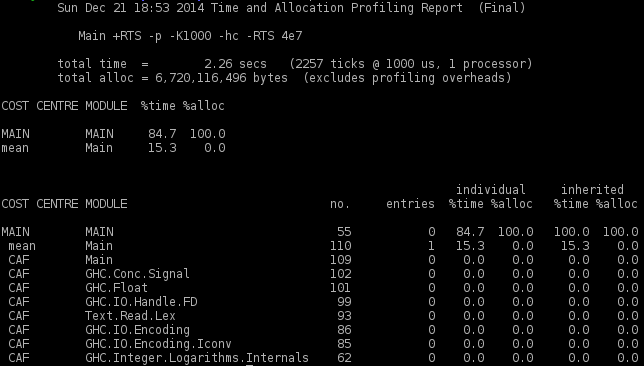
\includegraphics[width=\columnwidth]{images/profiler-placeholder}
  \footnotesize{Source: Made by the author.}
  \label{fig:profiler-sample}
\end{figure}

As we can see in this example, the first part of the report shows how the program was executed (which flags and arguments were passed to run it). Then, there is the total time and memory allocated during the whole execution of the program. The second part shows a break-down of the most costly cost centres.

\section{Criterion}\label{sec:criterion}
\lipsum[1-4]
